\documentclass[runningheads,a4paper]{llncs}
\usepackage{amssymb}
\setcounter{tocdepth}{3}
\usepackage{listings}
\usepackage{booktabs}
\usepackage{mathtools}
\usepackage{tabularx}
\usepackage{fixltx2e}
\PassOptionsToPackage{hyphens}{url}\usepackage{hyperref}
\usepackage[hyphens]{url}
\usepackage{upquote,textcomp}
\lstset{breaklines=true, basicstyle=\scriptsize\ttfamily, upquote=true}

\usepackage{fancyvrb}
\VerbatimFootnotes
\usepackage{cprotect}

\usepackage{graphicx}
\makeatletter
\def\maxwidth#1{\ifdim\Gin@nat@width>#1 #1\else\Gin@nat@width\fi}
\makeatother

\usepackage{amsmath}
\usepackage{pmml-new}

\usepackage{color,graphics,array,csscolor}

\usepackage{fontspec,unicode-math}
\usepackage[Latin,Greek]{ucharclasses}
\setTransitionsForGreek{\fontspec{Times New Roman}}{}

\usepackage{subscript}
\lstset{breaklines=true, basicstyle=\scriptsize\ttfamily}

\begin{document}
\mainmatter

\title{Network-based Knowledge Graph Assessment}

\author{Jan Rörden\inst{1} \and
Artem Revenko\inst{2} \and
Bernhard Haslhofer\inst{1} \and
Andreas Blumauer\inst{3}}
\authorrunning{Jan Rörden et al.}
\institute{Digital Insight Lab, Austrian Institute of Technology, Vienna, Austria\and
Semantic Web Company, Vienna, Austria\and
Semantic Web Company, Austria, Vienna\\
\email{jan.roerden@ait.ac.at, 
Artem.Revenko@semantic-web.com, 
Bernhard.Haslhofer@ait.ac.at, 
Andreas.Blumauer@semantic-web.com}}
\maketitle

\begin{abstract}
Knowledge graphs have become increasingly important in information retrieval tasks. However, if semantically interlinked concepts do not reflect the semantics of a document corpus, users might be confronted with non-relevant query results. In this work, we propose a network-metrics based method that allows assessment of knowledge graph quality within the context of a domain-specific document corpus. Preliminary results show that our methodology is able to point out structural and semantic issues in the knowledge graph, as well as provide information on the overall semantic fit of knowledge graph and domain specific corpora.
\end{abstract}


\section{Introduction}

A knowledge graph represents entities and their relations. Those entities - both abstract and concrete - can be grouped into classes according to their semantics, and should ideally cover every aspect that is important for a certain domain [Ehrlinger and Wöß, 2016]. Generally speaking, there are two different categories of knowledge graphs, generic and specific. Examples for generic graphs are DBpedia [Auer et al., 2007], the Google Knowledge Graph [Singhal, 2012] or Wikidata\footnote{\url{https://www.wikidata.org}}, which all cover a broad range of topics and domains. Specific knowledge graphs are tailored towards a specific domain, organization, or enterprise context.

Knowledge graphs often integrate data from various heterogeneous sources, provide a human-interpretable representation as well as a formalized, machine-readable basis for information retrieval tasks such as (latent) semantic indexing which relies on formalized and identifiable representation of real-world concepts [Deerwester et al., 1990], classification tasks and search engines or recommendation systems.

The effectiveness of those tasks heavily relies on the quality of the employed knowledge graph. Missing labeling and documentation issues can lead to misinterpretation, structural issues such as missing relationships between concepts might lead to incomplete or misleading interpretations of domain descriptions [Mader et al., 2012].

Related work in the area of knowledge graph quality (c.f., [Paulheim, 2017] for a survey), error detection and improvement studies has focused on the following issues: [Paulheim and Bizer, 2014] use statistical distributions of properties and types in RDF knowledge bases to compute their correctness; [Mader et al., 2012] and [Suominen and Mader, 2014] focus on SKOS vocabulary quality (e.g. missing/incomplete labels, orphan concepts, disconnected components) etc. Those and other methods rely on the knowledge graph itself. To our knowledge, there is no established research that uses a combined approach taking into account both a knowledge graph and a domain specific thesaurus (which is done for knowledge graph completion - but not for quality assessment).

In our work, we focus on knowledge graph quality issues that arise when the quality of a knowledge graph or thesaurus needs to be quantified in the context of a given document corpus, which is specific to a certain domain (e.g., medicine, economics). This requirement often arises when knowledge graph engineers or taxonomists take a document corpus as a basis for knowledge graph design or when existing graphs should be adapted to related application domains. Within this context, our contribution can be summarized as follows:
\begin{itemize}
\item We investigated the applicability of network metrics for measuring the quality of a given thesaurus in the context of a given, domain-specific document corpus.
\item We propose a method to quantify the semantic fit between thesaurus and document corpus.
\end{itemize}

Our proposed quality quantification methods should help taxonomists and domain experts, who are in charge of designing and managing a knowledge graph, to identify possible quality issues in their design and make informed decisions. Our poster will introduce this approach and accompanying demo will give visitors the opportunity to gain hands-on experience. 

\section{Approach}

Our network-based knowledge graph assessment approach consists of three subsequent steps: first, we apply a knowledge graph only perspective and compute network-based metrics to learn about the importance and structural relevance of concepts. Second, we focus on the document corpus and extract concepts and relationships using co-occurrence analysis techniques. Finally, we combine those two perspectives and provide metrics to assess the quality of a knowledge graph in the context of a document corpus.

\subsection{Knowledge Graph Perspective}

In a first step, we extract a network representation from given knowledge graphs expressed in SKOS by extracting skos:Concepts and a configurable set of SKOS\footnote{\url{https://www.w3.org/2004/02/skos/intro}} and non-SKOS relations.

By applying network clustering algorithms, we can identify unconnected components or concepts, which could be an indicator for missing relationships. We also compute the {\em diameter} of the knowledge graph, which might be an indicator for genericity or specificity of a knowledge graph. Figure 1 shows a network representation of the ``All about Cocktails'' thesaurus\footnote{ A thesaurus is a specific kind of knowledge graph that we use to demonstrate our method.}, with one concept being disconnected from the others. We will use this thesaurus as an example for the following metrics. Knowing which concepts occur both in the thesaurus and the corpus, we can also remove all concepts (vertices) from the thesaurus that are not mentioned in the corpus. The resulting graph can be quite different; so we use both the CG (corpus graph) and the TG (thesaurus graph) for further analysis.
\begin{figure}[h!]
\centering
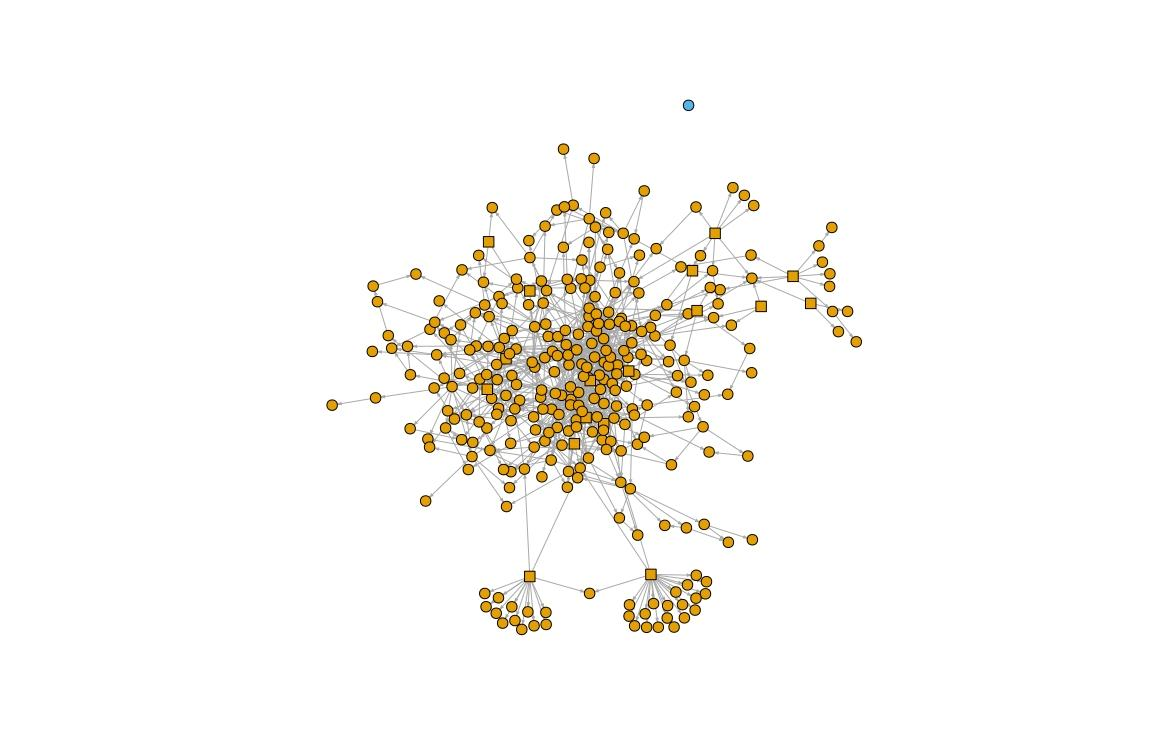
\includegraphics[width=\maxwidth{\textwidth}]{./img/image1.jpg}
\cprotect\caption{Network representation of a thesaurus}
\label{}
\end{figure}


On a concept-level, we compute the {\em degree} (number of incoming and outgoing edges) and {\em PageRank} of concepts, which can serve as indicators for the importance of a concept. Table 1 shows the {\em degree}, Table 2 the {\em PageRank}.
\begin{table}[h!]
\centering

\cprotect\caption{Concept degree}
\renewcommand{\tabularxcolumn}[1]{>{\arraybackslash}m{#1}}
\newcolumntype{Y}{>{\centering\arraybackslash}X}
\newcolumntype{Z}{>{\arraybackslash}X}

\scalebox{0.8} {\begin{tabularx}{1.22\textwidth}{ >{\hsize=0.5\hsize}Y  >{\hsize=0.5\hsize}Y }
\toprule

{\bf Concept label} & {\bf degree} \\
 \toprule

 „Martini glass`` & 34 \\
 \midrule

„Contemporary Classics`` & 31 \\
 \midrule

„The Unforgettables`` & 30 \\
 \midrule

„Gin`` & 24 \\
 \midrule

„Shooters`` & 22 \\
 \bottomrule

\end{tabularx}}

\label{}
\end{table}

\begin{table}[h!]
\centering

\cprotect\caption{Concept PageRank}
\renewcommand{\tabularxcolumn}[1]{>{\arraybackslash}m{#1}}
\newcolumntype{Y}{>{\centering\arraybackslash}X}
\newcolumntype{Z}{>{\arraybackslash}X}

\scalebox{0.8} {\begin{tabularx}{1.22\textwidth}{ >{\hsize=0.5\hsize}Y  >{\hsize=0.5\hsize}Y }
\toprule

{\bf Concept label} & {\bf PageRank} \\
 \toprule

„Martini glass`` & 0.0169 \\
 \midrule

„Old Tom Gin`` & 0.0121 \\
 \midrule

„Gin`` & 0.0114 \\
 \midrule

„Old Fashioned glass`` & 0.0110 \\
 \midrule

„Vodka Citron`` & 0.0109 \\
 \bottomrule

\end{tabularx}}

\label{}
\end{table}


By computing {\em closeness} (mean number of steps to access every other vertex) and {\em betweenness} (number of shortest paths going through a concept) of concepts, we can provide insight into the structural importance of concepts. Removing a concept with high {\em betweenness}, for example, could split a knowledge graph into several disconnected components.
\begin{table}[h!]
\centering

\cprotect\caption{Concept closeness}
\renewcommand{\tabularxcolumn}[1]{>{\arraybackslash}m{#1}}
\newcolumntype{Y}{>{\centering\arraybackslash}X}
\newcolumntype{Z}{>{\arraybackslash}X}

\scalebox{0.8} {\begin{tabularx}{1.22\textwidth}{ >{\hsize=0.5\hsize}Y  >{\hsize=0.5\hsize}Y }
\toprule

{\bf Concept label} & {\bf closeness} \\
 \toprule

„IBA official cocktails`` & 0.00854 \\
 \midrule

„Beverages`` & 0.00504 \\
 \midrule

„Contemporary Classics`` & 0.00499 \\
 \midrule

„The Unforgettables`` & 0.00462 \\
 \midrule

„Alcoholic beverages`` & 0.00437 \\
 \bottomrule

\end{tabularx}}

\label{}
\end{table}

\begin{table}[h!]
\centering

\cprotect\caption{Concept betweenness}
\renewcommand{\tabularxcolumn}[1]{>{\arraybackslash}m{#1}}
\newcolumntype{Y}{>{\centering\arraybackslash}X}
\newcolumntype{Z}{>{\arraybackslash}X}

\scalebox{0.8} {\begin{tabularx}{1.22\textwidth}{ >{\hsize=0.5\hsize}Y  >{\hsize=0.5\hsize}Y }
\toprule

{\bf Concept label} & {\bf betweenness} \\
 \toprule

„Distilled beverages`` & 0.00161 \\
 \midrule

„Liquer`` & 0.00124 \\
 \midrule

„Alcoholic beverages`` & 0.00088 \\
 \midrule

„Contemporary Classics`` & 0.00082 \\
 \midrule

„Vermouth`` & 0.00074 \\
 \bottomrule

\end{tabularx}}

\label{}
\end{table}


\subsection{Combined Knowledge Graph and Corpus Perspective }

The intuition behind this step is that a knowledge graph, which is a tailored to a specific domain, defines concepts and semantic relations, which should also appear in a document corpus taken from that domain.

As shown in Figure 2, possible discrepancies can already be observed by mapping corpus concepts onto a thesaurus network. This example shows a coverage of 81\% - green vertices (concepts) show up in both the thesaurus and the corpus.
\begin{figure}[h!]
\centering
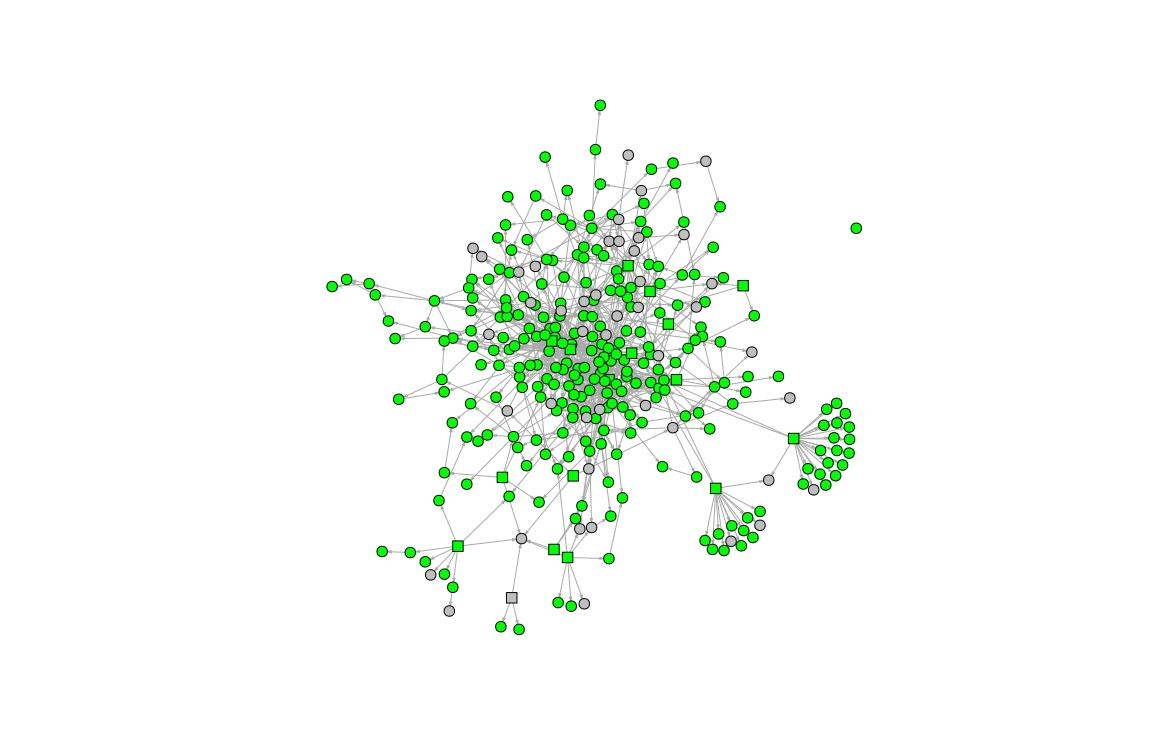
\includegraphics[width=\maxwidth{\textwidth}]{./img/image2.jpg}
\cprotect\caption{Thesaurus and corpus}
\label{}
\end{figure}


For the second part of our analysis, we go beyond simple coverage rate. Ideally, a thesaurus and a corpus share the same concepts\footnote{ The concepts have been extracted using the PoolParty API, which only returned the concepts that exist in the accompanying thesaurus.} and relations. The basic metrics are: number of distinct concepts; total concept occurrences; concept coverage (how many concepts of the thesaurus show up in the corpus?).  

Having gathered this information, we attempt to judge on how well a thesaurus fits a given corpus (or vice versa), going beyond simple concept coverage rate. For this, we calculated Pearson correlation coefficients between {\em document frequency} (df) of concepts on the one hand, and {\em PageRank}, {\em closeness} and {\em betweenness} on the other hand (Table 5).
\begin{table}[h!]
\centering

\cprotect\caption{Correlations}
\renewcommand{\tabularxcolumn}[1]{>{\arraybackslash}m{#1}}
\newcolumntype{Y}{>{\centering\arraybackslash}X}
\newcolumntype{Z}{>{\arraybackslash}X}

\scalebox{0.8} {\begin{tabularx}{1.22\textwidth}{ >{\hsize=0.33333333333333337\hsize}Y  >{\hsize=0.33333333333333337\hsize}Y  >{\hsize=0.33333333333333337\hsize}Y }
\toprule

{\bf Correlation} & {\bf Pearson correlation} & {\bf p-value} \\
 \toprule

df \& degree, TG & 0.165 & 0.006 \\
 \midrule

df \& degree, CG & 0.169 & 0.005 \\
 \midrule

df \& PageRank, TG  & 0.017 & 0.77 \\
 \midrule

df \& PageRank, CG & 0.036 & 0.55 \\
 \midrule

df \& betweenness, TG & 0.172 & 0.004 \\
 \midrule

df \& betweenness, CG & 0.175 & 0.003 \\
 \midrule

df \& closeness, TG & 0.130 & 0.03 \\
 \midrule

df \& closeness, CG & 0.111 & 0.06 \\
 \bottomrule

\end{tabularx}}

\label{}
\end{table}


Furthermore, we use {\em concept co-occurrences} as a measurement for semantic distance in the corpus, which we expect to be reflected in the thesaurus as well. For this, we perform a logarithmic transformation of co-occurrences to the range [1, thesaurusDiameter {\em d}]. The expectation here is that the higher the co-occurrence of any given pair of concepts is, the smaller should be their distance in the thesaurus. We apply cosine similarities of distance vectors to quantify the gap between optimal distances according to the co-occurrences and real distances based on the TG and the CG. A result of -1 means they are exactly opposite, 1 that they are the same and 0 indicates orthogonality:

\begin{equation}
\let\par\empty {\frac{{\left.\middle(d-{1}\middle)\middle({\frac{{{1}}}{{\left.log{\mi{}}\middle(x\middle){\mi{}}\right.}}}-min\middle({\frac{{{1}}}{{\left.log\middle(x\middle)\right.}}}\middle)\middle)\right.}}{{\left.max{\mi{}}\middle({\frac{{{1}}}{{\left.log{\mi{}}\middle(x\middle){\mi{}}\right.}}}\middle){\mi{}}-min\middle({\frac{{{1}}}{{\left.log\middle(x\middle)\right.}}}\middle)\right.}}}+{1}
\label{}
\end{equation}


This resulted in a cosine similarity of 0.80 for the complete thesaurus graph TG, and 0.77 for the corpus graph CG.

\subsection{Preliminary Results}

We have applied our methodology on a combination of 4 thesauri and 7 document corpora. Guided by our proposed metrics and combined with manual inspection, we were able to: 
\begin{itemize}
\item Find missing relationships between concepts, which were of semantic relevance in the corpus, but not reflected in the thesaurus.
\item Identify structural flaws in existing thesauri.
\item Map document corpora to specific regions of a thesaurus. This could be useful for creating domain-specific thesauri from generic knowledge graphs.
\end{itemize}

Currently, a clear limitation of our approach is that our proposed approach has not yet been evaluated against a gold-standard dataset. Therefore, we propose to implement the methodology presented here in a series of snapshots, triggered by the number of edits made. With this, domain experts can determine whether the concepts and relations they add have meaningful impact on the knowledge graphs quality.

\section{Demo Implementation}

The web application\footnote{\url{https://research.semantic-web.com/thesaurus\_harmony/}} allows one to connect to a PoolParty server, specify the project (thesaurus) and the related corpus, and assess the quality of their fit. The quality is assessed through the comparison of structural distances between concepts in the thesaurus versus the co-occurrence distances in the specified corpus ("Distances Comparison Quality"). The structural distance between individual pairs of concepts are plotted on the X axis, whereas textual distances are on the Y axis. The r\textasciicircum2 value of the linear approximation is taken as the score.

Moreover, the frequencies of the concepts in the corpus are depicted in the "taxonomy coverage" figure. With the help of the coverage figure the user can visualize and investigate the important concepts and branches in the thesaurus and, possibly, remove concepts or extend the most important branches. The occurring concepts are labelled blue, the concepts whose children occur in the corpus are marked orange, unmentioned concepts are gray.

In a separate ranking the user may investigate the "importance" of different concepts in the thesaurus. The importance is assessed with the help of betweenness metrics.

Another method for assessing the quality of the fit is called "information capture". Here the application plots the number of extracted concepts (Y axis) versus the importance score of the discovered terms (i.e. terms that are not present in the thesaurus). Since we struggle to annotate the document well and reflect the important information with the annotations, this figure helps to visualize how homogeneously the documents are annotated throughout the corpus. Again, the r\textasciicircum2 value of the linear approximation is taken as the score.

All the visualizations are interactive, the user may investigate the plots including zooming and getting informative tooltips.

\section{Conclusion and future work}

With the approach outlined in this paper, we are able to suggest improvements to the thesaurus so that it fits the corpus better. With the hypothesis that the distances from corpus-based co-occurrences and the thesaurus graph should be as congruent as possible, a number of improvements to a thesaurus can be made. Additionally, we implemented an initial proof-of-concept demo.

\subsection{Future Work}

We identified further possible improvements for our methodology, which will be implemented in a follow-up project later this year. Apart from improving the thesaurus by fixing obvious mistakes, we plan to re-create the thesaurus based on the corpus itself.

For this, we will use the semantic distances based on concept co-occurrences to re-create a network representation of a knowledge graph from scratch. The existing thesaurus can then either be improved (create and/or remove edges, only use a subset of a bigger thesaurus etc.), or the new graph can be enriched with additional information (vertex/edge type etc.) and used as a thesaurus; it could be even possible to combine existing thesauri. This approach is especially useful when the corpus is diverse and no fitting thesaurus exists.

\begin{thebibliography}{4}


Auer, Sören, et al. "Dbpedia: A nucleus for a web of open data." {\em The semantic web} (2007): 722-735.

Deerwester, Scott, et al. "Indexing by latent semantic analysis." {\em Journal of the American society for information science} 41.6 (1990): 391.

Ehrlinger, Lisa, and Wolfram Wöß. "Towards a Definition of Knowledge Graphs." {\em SEMANTiCS (Posters, Demos, SuCCESS)}. 2016.

Mader, Christian, Bernhard Haslhofer, and Antoine Isaac. "Finding quality issues in SKOS vocabularies." {\em Theory and Practice of Digital Libraries} (2012): 222-233. 

Paulheim, Heiko, and Christian Bizer. "Improving the quality of linked data using statistical distributions." {\em International Journal on Semantic Web and Information Systems (IJSWIS)} 10.2 (2014): 63-86. 

Paulheim, Heiko. "Knowledge graph refinement: A survey of approaches and evaluation methods." {\em Semantic web} 8.3 (2017): 489-508. 

Singhal, Amit. "Introducing the knowledge graph: things, not strings." {\em Official google blog} (2012).

Suominen, Osma, and Christian Mader. "Assessing and improving the quality of SKOS vocabularies." {\em Journal on Data Semantics} 3.1 (2014): 47-73.

\end{thebibliography}

\end{document}